\documentclass[11pt]{article}

%%%%%%%%%%%%      PACKAGES        %%%%%%%%%%%%
\usepackage[colorlinks=true,linkcolor=blue,urlcolor=blue,citecolor=blue]{hyperref}
\usepackage{setspace}
\onehalfspacing
%\doublespacing
\usepackage{fancyhdr,afterpage}
\usepackage{lscape}
\usepackage{multirow}
\usepackage{longtable}
\usepackage{textcomp,latexsym}
\usepackage{parskip}
\usepackage[round]{natbib}
\usepackage{adjustbox,lipsum}
\usepackage[titletoc]{appendix}
    
\usepackage[round]{natbib}
\usepackage{amsmath}
\usepackage{graphicx}
\usepackage{gensymb}
\usepackage{tikz}
\usepackage{float}
\usepackage{slashbox}
\usepackage{caption}
\usepackage{subcaption}
\usepackage{amsfonts}
\usepackage{enumerate}
\usepackage{amssymb}
\usepackage{multirow}
\usepackage{bm}
\setcounter{tocdepth}{3}
\setcounter{secnumdepth}{3}

\DeclareMathOperator*{\argmax}{arg\,max}
\DeclareMathOperator*{\argmin}{arg\,min}

\usepackage[a4paper,inner=4.2cm,outer=2.3cm,top=2.5cm,bottom=2.5cm,pdftex]{geometry} % MARGINS


\begin{document}
\section{Abstract}

\section{Introduction}

Most experiments are conducted in order to gain understanding of the impact that different parameters of interest make on the outcome; the quantitative measure of this impact allows comparisons as well as making interpretable conclusions regarding the scale and the pattern of the relationships between process parameters and measured output. 
%% Polynomial models
While the exact true nature of that relationship remains unknown, we need to have some form of approximation. Polynomial functions are well known to be able to provide an approximation of any required precision for functions from a certain class of differentiability \citep{Rudin1987real}: obviously, higher desirable precision would require a polynomial of a higher order and, therefore, more experimental effort. Response Surface Methodology (RSM) that was first introduced by \cite{Box1951Roy} is aimed at optimising the response by fitting a second order polynomial to the data obtained after an experiment on the points within the experimental region of interest has been performed. The response measured at each of $n$ experimental runs would then be presented as a linear combination of experimental factors' values, their interactions and corresponding quadratic terms; of course, some of the terms might be excluded, but, unless stated otherwise, we will consider a full second-order polynomial model with $1+2k+\frac{k(k-1)}{2}$ parameters (including the intercept), where $k$ is the number of factors. Together with the fixed polynomial part, the error term here would stand for all the variation in data that has not been captured by the model. 
%% Experimental design
At the stage of experimental planning, when there is little, if any, prior knowledge and no data available, there is still a lot that can and should be done to make sure the results of the experimentation and the following analysis are credible.

The design construction usually depends on the model in several ways. Firstly, the interest in the properties of the model parameters' estimation leads to the development of various optimality criteria (e.g.~so-called `alphabetic criteria'). Secondly, the fact of the model-dependence of the majority of the criteria implies the necessity of taking into account the possible lack-of-fit as well as the desirability of obtaining error variance estimates from replicated observations (model-independent, `pure' error). The latter two are also in the list of the properties of what would be considered as a `good design' (summarised by \cite{Box1987empirical}, Chapter $14$): it should ``make it possible to detect lack of fit'' and ``provide an internal estimate of error from replication''.

It is obvious that all the individual criteria are not interchangeable and can possibly be contradictory, however, they all are desired to be accounted for. There are a few ways of combining them, and here we will be working with the notion of a compound optimality criterion which is basically a weighted combination of the elementary criteria, where weights are generally arbitrary, and are expected to be chosen in accordance with the experimenter's beliefs and intentions. 

We will focus in this work on factorial experiments with a relatively small number of runs and the fitted model being a polynomial regression. We work here with exact designs: for each run we are to provide a point as a combination of the treatment factors' levels; therefore, finding the corresponding optimal design is essentially a matrix optimisation problem, i.e. searching for a design maximising (minimising) the criterion function. When considering examples of different compound criteria with various weight allocations, we will examine the resulting optimal designs in terms of their performances with respect to individual components. This would allow evaluating how much is ``lost'' when achieving a compromise, what component criteria contradict each others' performances, and how they are affected by changes of weight allocations.

The first and main objective of the research presented is to develop a methodology for combining several desirable data inference properties in compound optimality criteria for factorial experiments. The properties are to correspond to the precision of inference based on the primary model and to the possibility of the specified model contamination presence; the components are aimed to comply with the `pure error' strategy, where it is feasible.

The obvious following objective is to investigate the relationships between the individual components of the introduced criteria and, by considering some examples, provide some empirical recommendations for complex experimentation research that would benefit from applying these methods.

The criteria will also be adapted to be applied within experimental frameworks with restricted randomisation: blocked and multistratum experiments.

\section{Background}

Recall the polynomial regression model (\ref{eq::back_model}) for the unblocked experiment, containing initial factors, their powers and interactions is used as a good approximation to the relation between the variables:  

\begin{equation}
\label{eq::back_model}
\bm{Y}=\bm{X\beta}+\bm{\varepsilon}.
\end{equation} 

Here $\bm{X}$ is the $n\times p$ model matrix, $\bm{Y}$ is the $n\times 1$ vector of responses; $\bm{\beta}$ is the $p\times 1$ vector of parameters corresponding to the model terms and $\bm{\varepsilon}$ are independent normally distributed random error terms with constant variance, i.e. $\bm{\varepsilon}\sim \mathcal{N}(\bm{0},\sigma^{2}\bm{I}_{n})$.

\subsection{Pure error}
The error variance estimation can be obtained in two ways. The first one is the mean square error: $\hat{\sigma}^2_{mse}=\mbox{Residual SS}/(n-p)$, i.e. the residual sum of squares divided by the corresponding number of degrees of freedom (obtained from the ANOVA decomposition, the details can be found in \cite{Draper1998}). This estimator obviously depends on the model and on the number of its parameters. The other one is model-independent `pure' error, derived from the further decomposition of the residual sum of squares into the `pure' error and `lack-of-fit' components: $\hat{\sigma}^2_{PE}=\mbox{Pure error SS}/(n-t)$, where $t$ is the number of unique treatments applied and $d=n-t$ is the pure error degrees of freedom, i.e. the number of replicated points. In other words, the error is estimated by fitting the full treatment model:

\begin{equation}
\label{eq::back_trnt}
\bm{Y}=\bm{X_{t}\mu_{t}}+\bm{\varepsilon},
\end{equation} 

where $\bm{X_{t}}$ is the $n\times t$ full treatment model matrix, in which the $(i,j)^{th}$ element is equal to $1$ if treatment $j$ is applied to the $i^{th}$ unit, otherwise it is set to $0$. Then the elements of the $t$-dimensional vector $\bm{\mu_{t}}$ are the mean effects of each treatment. The vector of errors $\bm{\varepsilon}$ comprises the between-unit variation, such that $\mbox{E}(\bm{\varepsilon})=\bm{0}$, $\mbox{Var}(\bm{\varepsilon})=\sigma^2\bm{I}_{n}$.

Many authors advocate the use of the `pure' error estimate of $\sigma^2$ instead of the one pooled with the lack-of-fit part from the model (\ref{eq::back_model}): \cite{Cox1958planning} recommends using it for the estimation unless there are no replicate treatments, while \cite{Draper1998} argue for the reliability of `pure' error and recommend aiming for the presence of replicates at the stage of planning. \cite{Atkinson2007} also state that ``If lack-of-fit of the model is of potential interest, $\sigma^{2}$ is better estimated from replicate observations'' (page 22). For response surface experiments in blocks \cite{Gilmour2000PErsm} explicated the definition of pure error and its estimate which are compatible with the unblocked case: from replicates but also taking into account  block effects additive to treatment effects. Finally, the work by \cite{GilmourTrinca2012} that inspired this research, comprises a thorough analysis in favour of estimating the error from the full treatment model which is true regardless of what function is used to approximate the relationship of interest.


\subsection{Combining criteria}

The concept of the compound criteria is based on the notion of design efficiency, which can be defined for any design matrix and any criterion. For example, the $D$-efficiency of design $\bm{X}$ is
\begin{equation}
\label{eq::D_eff}
\mbox{Eff}_{D}(X)=\left[\frac{\vert \bm{X}'\bm{X}\vert}{\vert \bm{X}'_{*}\bm{X}_{*}\vert}\right]^{1/p},
\end{equation}   
where $\bm{X}_{*}$ is the $D$-optimum design. In this definition the power $1/p$ brings the efficiency to the scale of variances of model coefficients $\bm{\beta}_{i}, i=1\ldots p.$ It is obvious that the efficiency value may vary from $0$ to $1$ and is equal to $1$ if and only if the design is optimal according to the criterion of interest.

The final criterion function to be maximised among all the possible designs is obtained by combining the efficiencies for the component criteria $\mbox{Eff}_{1},\ldots, \mbox{Eff}_{m}$ with the corresponding weights $\kappa_{1},\ldots ,\kappa_{m}$ such that each $\kappa_{k}>0$ and $\sum_{k=1}^{m}\kappa_{k}=1:$

\begin{equation}
\label{eq::compound}
\mbox{Eff}^{\kappa_{1}}_{1}(\bm{X})\times\mbox{Eff}^{\kappa_{2}}_{2}(\bm{X})\times\ldots\times\mbox{Eff}^{\kappa_{m}}_{m}(\bm{X})\rightarrow \underset{\bm{X}}\max.
\end{equation}

The choice of weights is an arbitrary decision, made relying on both prior knowledge of the experimenter, the objectives of a specific experiment and the interpretation of the criterion components. The most general and intuitively sensible recommendation would be to obtain optimal designs with respect to several weight allocations, and then, after examining them, choose the one to be applied. Throughout the course of this research, when considering the examples of experiments layouts, we chose a set of weight allocations. Most of these sets were essentially classical design schemes for experiments with mixtures \citep{Cornell2011Mixtures}. For example, if the criterion consists of three elements, we would first obtain designs with all the weight on each component, then all combinations of distributing it equally between two components, and finally put equal weights on all of the components. Some additional schemes are included when examining particular cases.  

Some of the alternative approaches of considering several objectives would include the Pareto frontier approach, thoroughly described, for example, by \cite{Lu2011optimization}. When there are $l$ individual criterion functions $\phi_1(\bm{X}),\ldots\phi_{l}(\bm{X})$ to be maximised, the Pareto optimal set is generated so that for each of the designs from this set there is no other possible design that provides better criterion values for all the criteria (or, as it was defined, the Pareto optimal set is formed of designs that are not ``dominated'' by any other design).

Another approach was presented by \cite{Stallings2015general}: the authors developed methodology for generalising eigenvalue-based criteria (e.g. $A$- and $E$-optimality) in a way that allows differing interest (expressed through the weights) among any set of estimable functions of the fitted model parameters. The introduced strategy reflects the aims of experimentation that are not traditionally accounted for but definitely are of interest.

\section{Component criteria construction}
\label{ch::compound_criteria}
Standard design optimality theory is developed under the assumption that the fitted model represents the true relationship of interest and that there is no misspecification. However, it is obviously quite a strong belief and in reality we need to take into account at least the possibility that the model might not provide a good fit to the data. In Section \ref{sec::back_misspecification} a brief overview of various types of model misspecification is presented. 

In this chapter we consider the case when the fitted polynomial model is nested within a larger model that is assumed to provide a better fit for the data:
\begin{equation}
\label{eq::full_model}
\bm{Y}=\bm{X}_1\bm{\beta}_1+\bm{X}_2\bm{\beta}_2+\bm{\varepsilon},
\end{equation}
where $\bm{X}_2$ is an $n\times q$ is an extension of the initial model matrix representing those extra $q$ potential terms that might represent the fitted model disturbance. The vector $\bm{\beta}_2$ denotes the corresponding parameters. This larger model has $p+q$ parameters in total and not all of them are estimable when the experiment is relatively small: $n<p+q$; this is the case we consider here.
\subsection{Lack-of-fit criterion}
We consider the Generalised criterion presented by Goos et al.: [more details?]
\begin{equation*}
\mbox{minimise }|\bm{X}'_{1}\bm{X}_1|^{-\frac{\kappa_{D}}{p}}\times \left|\bm{L}+\frac{\bm{I}_{q}}{\tau^{2}}\right|^{-\frac{\kappa_{LoF}}{q}} \times |\bm{A}'\bm{A}+\bm{I}_{q}|.^{\frac{\kappa_{bias}}{q}},
\end{equation*}
where $\bm{L}$ is known in literature as dispersion matrix, and the matrix $\bm{L}+\bm{I}_{q}/\tau^{2}$ in the second component is essentially the inverse posterior variance-covariance matrix of the vector of potential terms (up to a factor of $\sigma^2$).

 ** Derivation first or the Generalised criterion

A diffuse prior shall be put on primary terms (as was done by \cite{DuMouchel1994}) -- an arbitrary mean and a variance going to infinity, and the prior on potential terms is the one specified before: $\bm{\beta}_2\sim\mathcal{N}(0,\bm{\Sigma}_{0})$,
$\bm{\Sigma}_{0}=\sigma^{2}\tau^{2}\bm{I}_{q}$, then the posterior
distribution of the coefficients is (as in \cite{Koch2007introduction} and \cite{DuMouchel1994}):
$$\bm{\beta}|\bm{Y}\sim \mathcal{N}(\bm{b},\bm{\Sigma}),\mbox{ where }\bm{b}=\bm{\Sigma X}'\bm{Y}, \bm{X}=[\bm{X}_1, \bm{X}_2],$$
$$\bm{\Sigma}=\left[\frac{\bm{K}}{\sigma^{2}\tau^{2}}+\sigma^{-2}(\bm{X'X})\right]^{-1}=\sigma^{2}[\bm{K}/\tau^{2}+\bm{X'}\bm{X}],^{-1}$$
and 
\begin{equation*}
\bm{K}=\begin{pmatrix}
\bm{0}_{p\times p} & \bm{0}_{p\times q}\\
\bm{0}_{q\times p} & \bm{I}_{q\times q}
\end{pmatrix}.
\end{equation*}
The marginal posterior of $\bm{\beta}_2$ is $\mathcal{N}(\bm{b}_{2},\bm{\Sigma}_{22})$, so using the general formula for the inverse of a block matrix
$$\begin{bmatrix}
 \bm{A}& \bm{B}\\
 \bm{C}& \bm{D}
\end{bmatrix}^{-1}=\begin{bmatrix}
\ldots & \ldots\\
\ldots & (\bm{D}-\bm{CA}^{-1}\bm{B})^{-1}
\end{bmatrix},$$
we can obtain the expression for $\bm{\Sigma}_{22}$:
\begin{align*}
[\bm{K}/\tau^{2}+\bm{X}'\bm{X}]^{-1}&=\begin{bmatrix}
 \bm{X}'_1\bm{X}_1& \bm{X}'_1\bm{X}_2 \\
 \bm{X}'_2\bm{X}_1& \bm{X}'_2\bm{X}_2+\bm{I}_{q}/\tau^{2}
\end{bmatrix}^{-1}\\&=\begin{bmatrix}
\ldots & \ldots\\
\ldots &
(\bm{X}'_2\bm{X}_2+\bm{I}_{q}/\tau^{2}-\bm{X}'_2\bm{X}_1(\bm{X}'_1\bm{X}_1)^{-1}\bm{X}'_1\bm{X}_2)^{-1}
\end{bmatrix},\\
\bm{\Sigma}_{22}&=\sigma^{2}[(\bm{K}/\tau^{2}+\bm{X}^{'}\bm{X})^{-1}]_{22}=\sigma^{2}\left(\bm{L}+\frac{\bm{I}_{q}}{\tau^{2}}\right)^{-1},
\end{align*} 
and $$(\bm{\Sigma}_{22})^{-1}=\frac{1}{\sigma^{2}}\left(\bm{L}+\frac{\bm{I}_{q}}{\tau^{2}}\right).$$

Therefore, the $(1-\alpha)\times100\%$ confidence region for the potential terms over the posterior distribution, when $\sigma^2$ is estimated by $s^2$ on $\nu$ degrees of freedom, is given by \citep{Draper1998}:

$$(\bm{\beta}_{2}-\bm{b}_{2})^{'}(\bm{L}+\bm{I}_{q}/\tau^{2})(\bm{\beta}_{2}-\bm{b}_{2})\leq qs^{2}F_{q,\nu;1-\alpha},$$
where $\mathrm{F}(q,\nu,\alpha)$ is the $\alpha$-quantile of F-distribution with $q$ and $\nu$ degrees of freedom.\\ 

\subsection{MSE-based bias criterion}
From the inference point of view, in the case of potential model contamination the bias in the parameters' estimates would be of substantial interest. A natural way of evaluating the quality of $\bm{\hat{\beta}}_{1}$, as noted by \citet{FedorovMontepiedra1997} is the matrix of  mean square error, which is the $\bm{L}_2$-distance between the true and estimated values with respect to the probability distribution measure of $\bm{Y}$ under the assumption of model (\ref{eq::full_m}):
\begin{align}
\label{eq::MSE}
\mbox{MSE}(\bm{\hat{\beta}}_1|\bm{\beta})=&\mathtt{E}_{\bm{Y}|\bm{\beta}}[(\bm{\hat{\beta}}_1-\bm{\beta}_1)(\bm{\hat{\beta}}_1-\bm{\beta}_1)']\notag\\=&\sigma^2(\bm{X}_1^{'}\bm{X}_1)^{-1}+\bm{A}\bm{\beta}_2\bm{\beta}_2'\bm{A}', 
\end{align}
where, as before, $\bm{A}=(\bm{X}_1^{'}\bm{X}_1)^{-1}\bm{X}_1^{'}\bm{X}_2$ is the alias matrix.
The determinant-based criterion function is minimising
\begin{equation}
\label{eq::MSE_det}
\mathtt{E}_{\beta}\log(\det[\mbox{MSE}(\bm{\hat{\beta}}_1|\bm{\beta})]),
\end{equation}
where by $\bm{\beta}$ we denote the joint vector of primary and potential model parameters: $\bm{\beta}=[\bm{\beta}_1, \bm{\beta}_2]$.
Using the matrix determinant lemma \citep{Harville2006matrix}
\begin{equation*}
\det[\bm{P}+\bm{uv}']=\det[\bm{P}]\det[1+\bm{v'}\bm{P}^{-1}\bm{u}], 
\end{equation*}
where $\bm{P}$ is an invertible square matrix and $\bm{u}$, $\bm{v}$ are column vectors, the determinant in (\ref{eq::MSE_det}) can be decomposed:
\begin{align}
\label{eq::mse_det_dec}
&\det[\mbox{MSE}(\bm{\hat{\beta}}_1|\bm{\beta}_2)]\notag\\&=\det[\sigma^2\bm{M}^{-1}+\bm{M}^{-1}\bm{X}_1^{'}\bm{X}_2\bm{\beta}_2\bm{\beta}_2'\bm{X}_2^{'}\bm{X}_1\bm{M}^{-1}]\notag\\&=\sigma^{2p}\det[\bm{M}^{-1}+\bm{M}^{-1}\bm{X}_1^{'}\bm{X}_2\bm{\tilde{\beta}}_2\bm{\tilde{\beta}}_2'\bm{X}_2^{'}\bm{X}_1\bm{M}^{-1}]\notag\\&=\sigma^{2p}\det[\bm{M}^{-1}]\det[1+\bm{\tilde{\beta}}_2'\bm{X}_2^{'}\bm{X}_1\bm{M}^{-1}\bm{M}\bm{M}^{-1}\bm{X}_1^{'}\bm{X}_2\bm{\tilde{\beta}}_2]\notag\\&=\sigma^{2p}\det[\bm{M}^{-1}](1+\bm{\tilde{\beta}}_2'\bm{X}_2^{'}\bm{X}_1\bm{M}^{-1}\bm{X}_1^{'}\bm{X}_2\bm{\tilde{\beta}}_2),\\
&\mbox{where } \bm{M}=\bm{X}_1^{'}\bm{X}_1 \mbox{ and }\bm{\tilde{\beta}}_2=\bm{\beta}_2/\sigma. \notag
\end{align}
Applying the logarithm function gives us the following sum:
\begin{align*}
&\log(\det[\mbox{MSE}(\bm{\hat{\beta}}_1|\bm{\beta}_2)])\\&=p\log\sigma^2+\log(\det[\bm{M}^{-1}])+\log(1+\bm{\tilde{\beta}}_2'\bm{X}_2^{'}\bm{X}_1\bm{M}^{-1}\bm{X}_1^{'}\bm{X}_2\bm{\tilde{\beta}}_2). 
\end{align*}
The first summand does not depend on the design, so it will not be included in the criterion; the second one is the $D$-optimality component. Therefore, (\ref{eq::MSE_det}) is replaced by
\begin{equation*}
\log(\det[\bm{M}^{-1}])+\mathtt{E}_{\bm{\tilde{\beta}}_2}\log(1+\bm{\tilde{\beta}}_2'\bm{X}_2^{'}\bm{X}_1\bm{M}^{-1}\bm{X}_1^{'}\bm{X}_2\bm{\tilde{\beta}}_2).
\end{equation*}

The second term needs to be evaluated numerically due to the obvious lack of information regarding the potential terms' coefficients. Note that as $\bm{\beta}_2 \sim \mathcal{N}(\bm{0},\tau^{2}\sigma^{2}\bm{I}_{q})$, then $\bm{\tilde{\beta}}_2 \sim \mathcal{N}(\bm{0},\tau^{2}\bm{I}_{q})$ and its prior distribution does not depend on the unknown $\sigma^2$.

To sum up, the resulting criterion function comprising the $DP$-criterion and the $LoF(DP)$-component from the generalised $DP$-criterion as well as the MSE-based part, all brought to the scale of efficiencies, is
\begin{align}
\label{eq::MSE_D}
\mbox{minimise }&\left[\left|\bm{X}'_{1}\bm{X}_{1}\right|^{-1/p}F_{p,d;1-\alpha_{DP}}\right]^{\kappa_{DP}} \times \notag \\ &\left[\left|\bm{L}+\frac{\bm{I}_{q}}{\tau^{2}}\right|^{-1/q}F_{q,d;1-\alpha_{LoF}}\right]^{\kappa_{LoF}}\times \notag\\ & \left[|\bm{X}'_{1}\bm{X}_{1}|^{-1}\exp\left(\frac{1}{N}\sum_{i=1}^{N}\log(1+\bm{\tilde{\beta}}_{2i}'\bm{X}_2^{'}\bm{X}_1\bm{M}^{-1}\bm{X}_1^{'}\bm{X}_2\bm{\tilde{\beta}}_{2i})\right)\right]_{.}^{\kappa_{MSE}/p}
\end{align}
Here $\bm{\tilde{\beta}}_{2i}$, $i=1..N$ -- independent random vectors sampled from $\mathcal{N}(\bm{0},\tau^{2}\sigma^{2}\bm{I}_{q})$.

\subsubsection{Point-based estimate}

One of the alternatives to the MC approach we would be willing to consider is to use the point prior for $\bm{\beta}_2$, that is $\bm{\beta}_2=\sigma\tau\bm{1}_q$ (where $\bm{1}_q$ is a $q$-dimensional vector with all components being equal to $1$), which is the standard deviation  of the initial (normal) prior. Therefore, $\bm{\tilde{\beta}}_2=\tau\bm{1}_q$, and the MSE(D)-part is
\begin{align*}
&|\bm{X}'_{1}\bm{X}_{1}|^{-1}(1+\bm{\tilde{\beta}}_{2}'\bm{X}_2^{'}\bm{X}_1\bm{M}^{-1}\bm{X}_1^{'}\bm{X}_2\bm{\tilde{\beta}}_{2})\\=&|\bm{X}'_{1}\bm{X}_{1}|^{-1}(1+\tau^2\bm{1}'_q\bm{X}_2^{'}\bm{X}_1\bm{M}^{-1}\bm{X}_1^{'}\bm{X}_2\bm{1}_q)\\=&|\bm{X}'_{1}\bm{X}_{1}|^{-1}\left(1+\tau^2\sum_{i,j=1}^{q}[\bm{X}_2^{'}\bm{X}_1\bm{M}^{-1}\bm{X}_1^{'}\bm{X}_2]_{(i,j)}\right),
\end{align*}
so essentially the last part of the equation is the summation of matrix elements, which obviously takes less computational time even for large dimensions $q$. 

The normal prior for $\bm{\beta}_2$ shall be preserved in the lack-of-fit component in (\ref{eq::MSE_D}), and so the criterion with the point prior estimate of the MSE(D)-component is the following function:
\begin{align}
\label{eq::MSE_D_point}
\mbox{minimise }&\left[\left|\bm{X}'_{1}\bm{X}_{1}\right|^{-1/p}F_{p,d;1-\alpha_{DP}}\right]^{\kappa_{DP}} \times \notag \\ &\left[\left|\bm{L}+\frac{\bm{I}_{q}}{\tau^{2}}\right|^{-1/q}F_{q,d;1-\alpha_{LoF}}\right]^{\kappa_{LoF}}\times \notag\\ & \left[|\bm{X}'_{1}\bm{X}_{1}|^{-1}\left(1+\tau^2\sum_{i,j=1}^{q}[\bm{X}_2^{'}\bm{X}_1\bm{M}^{-1}\bm{X}_1^{'}\bm{X}_2]_{(i,j)}\right)\right]_{.}^{\kappa_{MSE}/p}
\end{align}

Later we will refer to this as the ``MSE(D)P''-criterion, and in Section \ref{sec::mse_example} we will explore how much efficiency is lost when it is used instead of the computationally expensive original MSE(D)-based criterion (\ref{eq::MSE_D}).

To infer the trace-based form of the criterion, we use the pseudo-Bayesian approach to calculating the trace function of the MSE matrix (\ref{eq::MSE}): 
\begin{align*}
\mathtt{E}_{\beta_2}\mbox{trace}[\mbox{MSE}(\bm{\hat{\beta}}_1|\bm{\beta}_2)]&=\mbox{trace}[\mathtt{E}_{\beta_2}\mbox{MSE}(\bm{\hat{\beta}}_1|\bm{\beta}_2)]=\\&=\mbox{trace}[\sigma^2(\bm{X}_1^{'}\bm{X}_1)^{-1} + \mathtt{E}_{\bm{\beta}_2}(\bm{A}\bm{\beta}_2\bm{\beta}_2'\bm{A}')]=\\&=\mbox{trace}[\sigma^2(\bm{X}_1^{'}\bm{X}_1)^{-1}+\sigma^2\tau^2\bm{A}\bm{A}']=\\&=\sigma^2\mbox{trace}[(\bm{X}_1^{'}\bm{X}_1)^{-1}+\tau^2\bm{A}\bm{A}']\\&=\sigma^2[\mbox{trace}\{(\bm{X}_1^{'}\bm{X}_1)^{-1}\}+\tau^2\mbox{trace}\bm{A}\bm{A}'].
\end{align*}

The transitions above are possible due to commutativity of the operations of trace and expectation. The main advantage is the absence of the necessity of any additional numerical evaluations, and in this case of the trace-based criterion using the point prior for $\bm{\beta}_2$ defined earlier would lead to the same function. By minimising the whole function the sum of primary terms' variance and the expected squared norm of the bias vector in the direction of the potential terms are minimised simultaneously. The second part here contains the scaling parameter $\tau^2$ which regulates the magnitude of the potential terms' variation relatively to the error variance. 

Joining up the derived criterion function, the $LP$-criterion and the $LoF(LP)$-component from the generalised $LP$-criterion (\ref{eq::GLP_eff}), we obtain the compound criterion:
\begin{align}
\label{eq::MSE_L}
\mbox{minimise} &\left[\frac{1}{p}\mbox{trace}(\bm{WX}'_{1}\bm{X}_{1})^{-1}F_{1,d;1-\alpha_{LP}}\right]^{\kappa_{LP}}\times \notag\\& \left[\frac{1}{q}\mbox{trace}\left(\bm{L}+\frac{\bm{I}_{q}}{\tau^{2}}\right)^{-1}F_{1,d;1-\alpha_{LoF}}\right]^{\kappa_{LoF}}\times 
\notag\\& \left[\frac{1}{p}\mbox{trace}\{(\bm{X}'_{1}\bm{X}_{1})^{-1}+\tau^2\bm{A}\bm{A}'\}\right]^{\kappa_{MSE}}_{.}
\end{align}

\section{Examples}
\label{ch::compound_examples}

Here we will study the optimal designs in terms of the criteria (\ref{eq::MSE_D}), (\ref{eq::MSE_D_point}) and (\ref{eq::MSE_L}) (referred to as $MSE(D)$, $MSE(D)P$ and $MSE(L)$ criteria respectively) in the framework a factorial experiment, with $5$ factors, each is at three levels. The small number of runs ($40$) allows estimation of the full-second order polynomial model ($p=21$), but we assume that the `true' model contains also all third-order terms (linear-by-linear-by-linear and quadratic-by-linear interactions), $q=30$ of them in total.. 
[Some comparison with other criteria is to be added]

The intercept is a nuisance parameter, and so the criteria are adapted in such a way that the $DP$- and $LP$-components are replaced by $DPs$ and $LPs$. After considering the mean square error matrix (\ref{eq::MSE}) for $p-1$ parameters, in the MSE-based components the full information matrix is replaced by the one excluding the intercept -- $\bm{X}'_{1}\bm{Q}_0\bm{X}_{1}$ (see (\ref{eq::s_infmatrix})), where $\bm{X}_1$ is the model matrix without the intercept, $\bm{Q}_0=\bm{I}_n-\frac{1}{n}\bm{11}'$, and $\bm{\tilde{M}}$ is the full information matrix for the model with the intercept. Otherwise, the procedure of obtaining the $MSE(D)$- and $MSE(L)$-based components remains the same.

Below are expressions of the MSE-based criteria functions that have been amended according to the intercept exclusion from the set of parameters of interest:
\begin{align*}
\mbox{MSE(D): }&\left[\left|\bm{X}'_{1}\bm{Q}_0\bm{X}_{1}\right|^{-1/(p-1)}F_{p-1,d;1-\alpha_{DP}}\right]^{\kappa_{DP}} \times \notag \\ &\left[\left|\bm{L}+\frac{\bm{I}_{q}}{\tau^{2}}\right|^{-1/q}F_{q,d;1-\alpha_{LoF}}\right]^{\kappa_{LoF}}\times \notag\\ & \left[|\bm{X}'_{1}\bm{Q}_0\bm{X}_{1}|^{-1}\exp\left(\frac{1}{N}\sum_{i=1}^{N}\log(1+\bm{\tilde{\beta}}_{2i}'\bm{X}_2^{'}\bm{Q}_{0}\bm{X}_1\bm{\tilde{M}}^{-1}\bm{X}_1^{'}\bm{Q}_{0}\bm{X}_2\bm{\tilde{\beta}}_{2i})\right)\right]_{,}^\frac{\kappa_{MSE}}{(p-1)}
\end{align*}
\begin{align*}
\mbox{MSE(D)P:}&\left[\left|\bm{X}'_{1}\bm{Q}_0\bm{X}_{1}\right|^{-1/(p-1)}F_{p-1,d;1-\alpha_{DP}}\right]^{\kappa_{DP}} \times \notag \\ &\left[\left|\bm{L}+\frac{\bm{I}_{q}}{\tau^{2}}\right|^{-1/q}F_{q,d;1-\alpha_{LoF}}\right]^{\kappa_{LoF}}\times \notag\\ & \left[|\bm{X}'_{1}\bm{Q}_0\bm{X}_{1}|^{-1}\left(1+\tau^2\sum_{i,j=1}^{q}[\bm{X}_2^{'}\bm{Q}_{0}\bm{X}_1\bm{\tilde{M}}^{-1}\bm{X}_1^{'}\bm{Q}_{0}\bm{X}_2]_{(i,j)}\right)\right]_{,}^\frac{\kappa_{MSE}}{(p-1)}\\
\mbox{MSE(L):} &\left[\frac{1}{p}\mbox{trace}(\bm{WX}'_{1}\bm{Q}_{0}\bm{X}_{1})^{-1}F_{1,d;1-\alpha_{LP}}\right]^{\kappa_{LP}}\times \notag\\& \left[\frac{1}{q}\mbox{trace}\left(\bm{L}+\frac{\bm{I}_{q}}{\tau^{2}}\right)^{-1}F_{1,d;1-\alpha_{LoF}}\right]^{\kappa_{LoF}}\times 
\notag\\& \left[\frac{1}{p-1}\mbox{trace}\{\bm{\tilde{M}}^{-1}+\tau^2\bm{A}\bm{A}'\}_{22}\right]_{.}^{\kappa_{MSE}}
\end{align*}

In the third component of the MSE(L)-criterion the $\{\bm{\tilde{M}}^{-1}+\tau^2\bm{A}\bm{A}'\}_{22}$ stands for the submatrix corresponding to the parameters of interest, i.e.~the first column and the first row are to be excluded. It is worth noting that these criteria are a special case of a blocked experiment framework (with one block), which will be explicitly described in the next chapter.

Considering two values of the variance scaling parameter $\tau^2=1$ and $\tau^2=1/q$, for each compound criterion we obtain two sets of optimal designs, given in Tables \ref{tab::MSE(D)_ex1}, \ref{tab::MSE(L)_ex1} and \ref{tab::MSE(D)P_ex1}. 

The first three columns of the tables contain information about the weight distribution among the criterion components, so that every row corresponds to the design that has been obtained as optimal according to the criterion with the given weights. The next two columns show how the available residual degrees of freedom were allocated between the pure error and lack-of-fit components. Finally, the efficiencies of the resulting designs with respect to the individual criterion components are given in the last columns. In the case of the $MSE(D)P$-optimal designs, in Table \ref{tab::MSE(D)P_ex1}, the difference between their $MSE(D)$-efficiency values and the $MSE(D)$-efficiencies of the corresponding designs in Table \ref{tab::MSE(D)_ex1} indicates how much we lose in terms of the performance when the point prior is used for the $MSE(D)$-component estimation. 

It is worth noting that when this criterion part is being estimated using a stochastic method (MC in this case), despite the error being small, the efficiency values are still approximate. Another disadvantage is the increased time consumption of the algorithm in comparison to the previously considered criteria: with $150$ random starts, it can take up to several days to obtain an $MSE(D)$-optimal design; whilst $MSE(D)P$- and $MSE(L)$-based optimal designs are usually obtained within $4$--$8$ hours, even with $500$ random starts. 

%%% MSE(D) designs, tau^2=1 and tau^2=1/q
\begin{table}[h]
\caption{Properties of MSE(D)-optimal designs}
\label{tab::MSE(D)_ex1}
\resizebox{\textwidth}{!}}                               \\
   & \textbf{DP}       & \textbf{LoF(DP)}    & \textbf{MSE(D)}   & \textbf{PE}        & \textbf{LoF}        & \textbf{DP}   & \textbf{LoF(DP)}   & \textbf{MSE(D)}  &  \textbf{LP}       & \textbf{LoF(LP)}   & \textbf{MSE(L)}  \\
1 & 1    & 0    & 0    & \multicolumn{1}{|r}{18} & \multicolumn{1}{r|}{1}  & 100.00 & 47.77  & 91.05  & \multicolumn{1}{|r}{96.38} & 94.92 & 10.70 \\
2 & 0    & 1    & 0    & \multicolumn{1}{|r}{8}  & \multicolumn{1}{r|}{11} & 43.70  & 100.00 & 54.74  & \multicolumn{1}{|r}{0.75}  & 89.99 & 2.08  \\
3 & 0    & 0    & 1    & \multicolumn{1}{|r}{0}  & \multicolumn{1}{r|}{19} & 0.00   & 0.00   & 100.00 & \multicolumn{1}{|r}{0.00}  & 0.00  & 22.32 \\
4 & 0.5  & 0.5  & 0    & \multicolumn{1}{|r}{11} & \multicolumn{1}{r|}{8}  & 78.50  & 87.61  & 88.56  & \multicolumn{1}{|r}{73.88} & 98.85 & 17.66 \\
5 & 0.5  & 0    & 0.5  & \multicolumn{1}{|r}{15} & \multicolumn{1}{r|}{4}  & 97.26  & 56.51  & 93.77  & \multicolumn{1}{|r}{97.55} & 50.04 & 12.74 \\
6 & 0    & 0.5  & 0.5  & \multicolumn{1}{|r}{8}  & \multicolumn{1}{r|}{11} & 64.72  & 96.84  & 87.53  & \multicolumn{1}{|r}{57.04} & 36.17 & 29.33 \\
7 & 1/3  & 1/3  & 1/3  & \multicolumn{1}{|r}{10} & \multicolumn{1}{r|}{9}  & 79.45  & 84.14  & 93.23  & \multicolumn{1}{|r}{81.06} & 43.42 & 16.71 \\
8 & 0.5  & 0.25 & 0.25 & \multicolumn{1}{|r}{13} & \multicolumn{1}{r|}{6}  & 93.38  & 64.35  & 95.55  & \multicolumn{1}{|r}{95.76} & 48.58 & 14.77 \\
9 & 0.25 & 0.5  & 0.25 & \multicolumn{1}{|r}{9} & \multicolumn{1}{r|}{10} & 69.52  & 95.76  & 87.36  & \multicolumn{1}{|r}{63.13} & 40.41 & 25.46 \\
 & & & & & & & & & & & \\
   & \multicolumn{3}{l}{\textbf{Criteria, $\bm{\tau^2=1/q$}}} & \multicolumn{2}{l}{\textbf{DoF}} & \multicolumn{6}{l}{\textbf{Efficiency,\%}}                               \\
   & \textbf{DP}       & \textbf{LoF(DP)}    & \textbf{MSE(D)}   & \textbf{PE}        & \textbf{LoF}        & \textbf{DP}   & \textbf{LoF(DP)}   & \textbf{MSE(D)}  & \textbf{LP}       & \textbf{LoF(LP)}   & \textbf{MSE(L)}  \\
1 & 1    & 0    & 0    & \multicolumn{1}{|r}{18} & \multicolumn{1}{r|}{1}  & 100.00 & 94.41  & 90.60  & \multicolumn{1}{|r}{96.42} & 98.36  & 44.94 \\
2 & 0    & 1    & 0    & \multicolumn{1}{|r}{16} & \multicolumn{1}{r|}{3}  & 39.66  & 100.00 & 37.95  & \multicolumn{1}{|r}{0.13}  & 100.00 & 0.12  \\
3 & 0    & 0    & 1    & \multicolumn{1}{|r}{0}  & \multicolumn{1}{r|}{19} & 0.00   & 0.00   & 100.00 & \multicolumn{1}{|r}{0.00}  & 0.00   & 77.97 \\
4 & 0.5  & 0.5  & 0    & \multicolumn{1}{|r}{18} & \multicolumn{1}{r|}{1}  & 100.00 & 94.41  & 90.60  & \multicolumn{1}{|r}{96.42} & 98.36  & 44.94 \\
5 & 0.5  & 0    & 0.5  & \multicolumn{1}{|r}{17} & \multicolumn{1}{r|}{2}  & 97.31  & 91.28  & 93.98  & \multicolumn{1}{|r}{96.21} & 94.32  & 50.53 \\
6 & 0    & 0.5  & 0.5  & \multicolumn{1}{|r}{15} & \multicolumn{1}{r|}{4}  & 96.10  & 92.31  & 93.29  & \multicolumn{1}{|r}{99.48} & 95.09  & 57.05 \\
7 & 1/3  & 1/3  & 1/3  & \multicolumn{1}{|r}{18} & \multicolumn{1}{r|}{1}  & 100.00 & 94.41  & 90.60  & \multicolumn{1}{|r}{96.42} & 98.36  & 44.94 \\
8 & 0.5  & 0.25 & 0.25 & \multicolumn{1}{|r}{18} & \multicolumn{1}{r|}{1}  & 100.00 & 94.41  & 90.60  & \multicolumn{1}{|r}{96.42} & 98.36  & 44.94 \\
9 & 0.25 & 0.5  & 0.25 & \multicolumn{1}{|r}{18} & \multicolumn{1}{r|}{1}  & 99.96  & 94.33  & 90.65  & \multicolumn{1}{|r}{96.24} & 98.31  & 44.84 
\end{tabular}
}
\end{table}

The resulting designs tend to have a lot of the available degrees of freedom allocated to the pure error, except, for example, for the $MSE(D)$-optimal designs (\#$3$). However, for the smaller value of $\tau^2=1/q$ the imbalance is more extreme for the determinant-based criteria, where almost no degrees of freedom are left for lack of fit.

There are no repeated designs for $\tau^2=1$, but for $\tau^2=1/q$, in Table \ref{tab::MSE(D)_ex1}, designs \#$4$, \#$7$ and \#$8$ are the same as the $DP$-optimal design, and have quite large values of other efficiencies, and design \#$9$, although it is different, has quite similar efficiency values. 

The $DP$-optimal design is given in Table \ref{tab::DP_design}; it performs well in terms of the $MSE(D)$-component for both values of $\tau^2$, however, its $LoF(DP)$-efficiency drops by roughly half when the scaling parameter goes from $1/q$ to $1$; also, $LoF(DP)$-optimal designs provide the lowest $DP$-efficiency values (around $40\%$) for any value of $\tau^2$.

\begin{table}[h]
\centering
\caption{MSE(D)-criterion, DP-optimal design}
\label{tab::DP_design}
\scalebox{0.8}{
\begin{tabular}{rrrrrr|r|rrrrrr}
1  & -1 & -1 & -1 & -1 & -1 &  & 21 & 0 & -1 & -1 & 1  & 0  \\
2  & -1 & -1 & -1 & -1 & -1 &  & 22 & 0 & 0  & 0  & -1 & 1  \\
3  & -1 & -1 & 0  & 1  & 1  &  & 23 & 0 & 0  & 0  & -1 & 1  \\
4  & -1 & -1 & 1  & -1 & 1  &  & 24 & 0 & 1  & -1 & 0  & -1 \\
5  & -1 & -1 & 1  & -1 & 1  &  & 25 & 1 & -1 & -1 & -1 & 1  \\
6  & -1 & -1 & 1  & 1  & -1 &  & 26 & 1 & -1 & -1 & -1 & 1  \\
7  & -1 & -1 & 1  & 1  & -1 &  & 27 & 1 & -1 & -1 & 1  & -1 \\
8  & -1 & 0  & -1 & 0  & 1  &  & 28 & 1 & -1 & -1 & 1  & -1 \\
9  & -1 & 0  & -1 & 0  & 1  &  & 29 & 1 & -1 & 1  & -1 & -1 \\
10 & -1 & 1  & -1 & -1 & 1  &  & 30 & 1 & -1 & 1  & -1 & -1 \\
11 & -1 & 1  & -1 & -1 & 1  &  & 31 & 1 & -1 & 1  & 1  & 1  \\
12 & -1 & 1  & -1 & 1  & -1 &  & 32 & 1 & -1 & 1  & 1  & 1  \\
13 & -1 & 1  & -1 & 1  & -1 &  & 33 & 1 & 0  & -1 & -1 & 0  \\
14 & -1 & 1  & 0  & 0  & 0  &  & 34 & 1 & 1  & -1 & -1 & -1 \\
15 & -1 & 1  & 0  & 0  & 0  &  & 35 & 1 & 1  & -1 & 1  & 1  \\
16 & -1 & 1  & 1  & -1 & -1 &  & 36 & 1 & 1  & -1 & 1  & 1  \\
17 & -1 & 1  & 1  & -1 & -1 &  & 37 & 1 & 1  & 1  & -1 & 1  \\
18 & -1 & 1  & 1  & 1  & 1  &  & 38 & 1 & 1  & 1  & -1 & 1  \\
19 & -1 & 1  & 1  & 1  & 1  &  & 39 & 1 & 1  & 1  & 1  & -1 \\
20 & 0  & -1 & -1 & 1  & 0  &  & 40 & 1 & 1  & 1  & 1  & -1
\end{tabular}
}
\end{table}

As for the trace-based criterion and the optimal designs studied in Table \ref{tab::MSE(L)_ex1}, in general, all of them tend to have larger $LP$- and $MSE(L)$-efficiencies in case of smaller $\tau^2$, i.e. the decreased scale of the potentially missed contamination results in a more easily achievable compromise between the contradicting parts of the criteria (the same happens with the trace-based efficiencies of the MSE determinant-based optimal designs). It is also notable that, as it was observed in the case of generalised criteria, the $LoF(LP)$-optimal design is also $LoF(DP)$-optimal for $\tau^2=1/q$ (design \#$2$ in the corresponding tables).

The $MSE(L)$-component seems to be much more sensitive to the weight allocations than the $MSE(D)$ component. For example, in the case of $\tau^2=1$ some decent efficiency values are gained only when the whole weight is on the `potential terms' criterion components, i.e.~designs \#$3$ and \#$6$. 

It does not seem to work agreeably with the $LoF(LP)$-component either: the $LoF(LP)$-optimal design is $0.00\%$ $LP$- and $MSE(L)$-efficient in the case of $\tau^2=1$, and the efficiencies are close to $0\%$ in the case of smaller $\tau^2$. 
%% MSE(L) criteria
\begin{table}[h]
\caption{Properties of MSE(L)-optimal designs}
\label{tab::MSE(L)_ex1}
\resizebox{\textwidth}{!}}                               \\
   & \textbf{LP}       & \textbf{LoF(LP)}    & \textbf{MSE(L)}   & \textbf{PE}        & \textbf{LoF}        & \textbf{DP}   & \textbf{LoF(DP)}   & \textbf{MSE(D)}  &  \textbf{LP}       & \textbf{LoF(LP)}   & \textbf{MSE(L)}  \\
1 & 1    & 0    & 0    & \multicolumn{1}{|r}{16} & \multicolumn{1}{r|}{3} & 97.54 & 53.86 & 92.54 & \multicolumn{1}{|r}{100.00} & 96.87  & 12.08  \\
2 & 0    & 1    & 0    & \multicolumn{1}{|r}{13} & \multicolumn{1}{r|}{6} & 35.43 & 81.99 & 36.72 & \multicolumn{1}{|r}{0.00}   & 100.00 & 0.00   \\
3 & 0    & 0    & 1    & \multicolumn{1}{|r}{4} & \multicolumn{1}{r|}{15} & 18.67 & 38.43 & 51.84 & \multicolumn{1}{|r}{11.73}  & 34.79  & 100.00 \\
4 & 0.5  & 0.5  & 0    & \multicolumn{1}{|r}{15} & \multicolumn{1}{r|}{4} & 95.14 & 60.37 & 92.78 & \multicolumn{1}{|r}{99.80}  & 98.12  & 13.99  \\
5 & 0.5  & 0    & 0.5  & \multicolumn{1}{|r}{12} & \multicolumn{1}{r|}{7} & 77.77 & 72.05 & 84.91 & \multicolumn{1}{|r}{81.10}  & 98.72  & 25.19  \\
6 & 0    & 0.5  & 0.5  & \multicolumn{1}{|r}{9} & \multicolumn{1}{r|}{10} & 36.80 & 70.91 & 51.12 & \multicolumn{1}{|r}{28.13}  & 91.60  & 83.52  \\
7 & 1/3  & 1/3  & 1/3  & \multicolumn{1}{|r}{11} & \multicolumn{1}{r|}{8} & 69.53 & 73.16 & 79.71 & \multicolumn{1}{|r}{70.59}  & 97.47  & 27.98  \\
8 & 0.5  & 0.25 & 0.25 & \multicolumn{1}{|r}{12} & \multicolumn{1}{r|}{7} & 77.20 & 72.83 & 84.44 & \multicolumn{1}{|r}{81.47}  & 98.80  & 23.88  \\
9 & 0.25 & 0.5  & 0.25 & \multicolumn{1}{|r}{12} & \multicolumn{1}{r|}{7} & 70.90 & 69.80 & 78.15 & \multicolumn{1}{|r}{72.16}  & 98.49  & 26.19  \\
 & & & & & & & & & & & \\
   & \multicolumn{3}{l}{\textbf{Criteria, $\bm{\tau^2=1/q$}}} & \multicolumn{2}{l}{\textbf{DoF}} & \multicolumn{6}{l}{\textbf{Efficiency,\%}}                               \\
   & \textbf{LP}       & \textbf{LoF(LP)}    & \textbf{MSE(L)}   & \textbf{PE}        & \textbf{LoF}        & \textbf{DP}   & \textbf{LoF(DP)}   & \textbf{MSE(D)}  & \textbf{LP}       & \textbf{LoF(LP)}   & \textbf{MSE(L)}  \\
1 & 1    & 0    & 0    & \multicolumn{1}{|r}{16} & \multicolumn{1}{r|}{3} & 97.54 & 92.13 & 92.18 & \multicolumn{1}{|r}{100.00} & 95.61  & 52.55  \\
2 & 0    & 1    & 0    & \multicolumn{1}{|r}{16} & \multicolumn{1}{r|}{3} & 39.66 & 100.00 & 37.95 & \multicolumn{1}{|r}{0.13}   & 100.00 & 0.12   \\
3 & 0    & 0    & 1    & \multicolumn{1}{|r}{3} & \multicolumn{1}{r|}{16} & 0.77  & 0.93  & 83.48 & \multicolumn{1}{|r}{0.02}   & 0.01   & 100.00 \\
4 & 0.5  & 0.5  & 0    & \multicolumn{1}{|r}{17} & \multicolumn{1}{r|}{2} & 96.87 & 94.29 & 89.84 & \multicolumn{1}{|r}{97.97}  & 97.80  & 51.17  \\
5 & 0.5  & 0    & 0.5  & \multicolumn{1}{|r}{12} & \multicolumn{1}{r|}{7} & 79.66 & 87.18 & 86.32 & \multicolumn{1}{|r}{84.81}  & 88.22  & 79.60  \\
6 & 0    & 0.5  & 0.5  & \multicolumn{1}{|r}{13} & \multicolumn{1}{r|}{6} & 76.46 & 89.87 & 80.78 & \multicolumn{1}{|r}{79.23}  & 91.48  & 79.11  \\
7 & 1/3  & 1/3  & 1/3  & \multicolumn{1}{|r}{13} & \multicolumn{1}{r|}{6} & 81.53 & 90.09 & 85.52 & \multicolumn{1}{|r}{85.96}  & 91.56  & 76.65  \\
8 & 0.5  & 0.25 & 0.25 & \multicolumn{1}{|r}{15} & \multicolumn{1}{r|}{4} & 90.60 & 91.94 & 88.43 & \multicolumn{1}{|r}{95.09}  & 94.75  & 63.82  \\
9 & 0.25 & 0.5  & 0.25 & \multicolumn{1}{|r}{15} & \multicolumn{1}{r|}{4} & 84.12 & 92.88 & 83.39 & \multicolumn{1}{|r}{87.86}  & 95.51  & 72.66 
\end{tabular}
}
\end{table}

Regarding the designs' performances with respect to the $DP$- and $LP$-components, it can be observed that the designs tend to be quite $DP$-efficient, overall more efficient in the case of $MSE(D)$-efficient designs with smaller $\tau^2$. $DP$-efficient designs are not bad in terms of $LP$-efficiency and vice versa; again, the same cannot be said for the lack-of-fit components and seems not to be true at all for the $MSE$ components, especially, for the $MSE(L)$-optimal design when $\tau^2=1$.
   
$LP$- and $MSE(L)$-components seem to be in a conflict, though for $\tau^2=1/q$ $MSE(L)$-efficiency values are stable across the designs, therefore, making it possible to find compromise designs which at least perform not too badly with regard to both of these criterion parts; for example, designs \#$5$ -- \#$7$ are more than $75\%$-efficient (Table \ref{tab::MSE(L)_ex1}).   

Table \ref{tab::MSE(D)P_ex1} provides the performance summary of the designs constructed in the same way as the designs given in Table \ref{tab::MSE(D)_ex1}, but with the point prior of $\bm{\beta}_2=\sigma\tau\bm{1}_q$ used for the estimation of the $MSE(D)$-component of the criterion. This approach allowed reducing the computational times considerably, from as long as $2$ days to just a few hours, with other parameters being equal.

%%% MSE(D) criteria, point prior on beta2 !!!
\begin{table}[h]
\caption{Properties of MSE(D)-optimal designs, with point prior}
\label{tab::MSE(D)P_ex1}
\resizebox{\textwidth}{!}}                               \\
   & \textbf{DP}       & \textbf{LoF(DP)}    & \textbf{MSE(D)P}  & \textbf{PE}        & \textbf{LoF}        & \textbf{DP}   & \textbf{LoF(DP)}   & \textbf{MSE(D)}  & \textbf{MSE(D)P} &  \textbf{LP}       & \textbf{LoF(LP)}   & \textbf{MSE(L)}  \\
1 & 1    & 0    & 0 & \multicolumn{1}{|r}{18} & \multicolumn{1}{r|}{1} & 100.00 & 47.77 & 91.05 & \multicolumn{1}{|r}{90.06} & \multicolumn{1}{|r}{96.38} & 94.92 & 10.70 \\
2 & 0    & 1    & 0 & \multicolumn{1}{|r}{8} & \multicolumn{1}{r|}{11} & 43.70 & 100.00 & 54.74 & \multicolumn{1}{|r}{53.51} & \multicolumn{1}{|r}{0.75} & 89.99 & 2.08  \\
3 & 0    & 0    & 1 & \multicolumn{1}{|r}{0} & \multicolumn{1}{r|}{19} & 0.00 & 0.00 & 98.18 & \multicolumn{1}{|r}{100.00} & \multicolumn{1}{|r}{0.00} & 0.00 & 23.72 \\
4 & 0.5  & 0.5  & 0    & \multicolumn{1}{|r}{11} & \multicolumn{1}{r|}{8} & 78.50 & 87.61 & 88.56 & \multicolumn{1}{|r}{87.04} & \multicolumn{1}{|r}{73.88} & 98.85 & 17.66 \\
5 & 0.5  & 0    & 0.5  & \multicolumn{1}{|r}{18} & \multicolumn{1}{r|}{1} & 100.00 & 47.77 & 90.70 & \multicolumn{1}{|r}{93.28} & \multicolumn{1}{|r}{96.38} & 94.92 & 10.70 \\
6 & 0    & 0.5  & 0.5  & \multicolumn{1}{|r}{8} & \multicolumn{1}{r|}{11} & 65.84 & 94.78 & 88.51 & \multicolumn{1}{|r}{88.72} & \multicolumn{1}{|r}{58.15} & 89.54 & 23.63 \\
7 & 1/3  & 1/3  & 1/3  & \multicolumn{1}{|r}{11} & \multicolumn{1}{r|}{8} & 83.32 & 80.22 & 92.71 & \multicolumn{1}{|r}{94.22} & \multicolumn{1}{|r}{84.52} & 98.34 & 17.21 \\
8 & 0.5  & 0.25 & 0.25 & \multicolumn{1}{|r}{13} & \multicolumn{1}{r|}{6} & 92.07 & 66.67 & 94.27 & \multicolumn{1}{|r}{94.92} & \multicolumn{1}{|r}{94.02} & 98.91 & 13.88 \\
9 & 0.25 & 0.5  & 0.25 & \multicolumn{1}{|r}{9} & \multicolumn{1}{r|}{10} & 69.69  & 95.64  & 87.48 & \multicolumn{1}{|r}{86.46}  & \multicolumn{1}{|r}{61.06} & 94.29 & 25.30 \\
 & & & & & & & & & & & & \\
   & \multicolumn{3}{l}{\textbf{Criteria, $\bm{\tau^2=1/q}$}} & \multicolumn{2}{l}{\textbf{DoF}} & \multicolumn{6}{l}{\textbf{Efficiency,\%}}                               \\
   & \textbf{DP}       & \textbf{LoF(DP)}    & \textbf{MSE(D)P} & \textbf{PE}        & \textbf{LoF}        & \textbf{DP}   & \textbf{LoF(DP)}   & \textbf{MSE(D)} & \textbf{MSE(D)P} & \textbf{LP}       & \textbf{LoF(LP)}   & \textbf{MSE(L)}  \\
1 & 1    & 0    & 0    & \multicolumn{1}{|r}{18} & \multicolumn{1}{r|}{1} & 100.00 & 94.41  & 90.60 & \multicolumn{1}{|r}{90.23}  & \multicolumn{1}{|r}{96.42} & 98.36 & 44.94 \\
2 & 0    & 1    & 0    & \multicolumn{1}{|r}{16} & \multicolumn{1}{r|}{3} & 39.66  & 100.00 & 37.95 & \multicolumn{1}{|r}{37.87}  & \multicolumn{1}{|r}{0.13}  & 100.00 & 0.12  \\
3 & 0    & 0    & 1    & \multicolumn{1}{|r}{0} & \multicolumn{1}{r|}{19} & 0.00   & 0.00   & 98.30 & \multicolumn{1}{|r}{100.00} & \multicolumn{1}{|r}{0.00}  & 0.00  & 77.96 \\
4 & 0.5  & 0.5  & 0    & \multicolumn{1}{|r}{18} & \multicolumn{1}{r|}{1}  & 100.00 & 94.41  & 90.60 & \multicolumn{1}{|r}{90.23}  & \multicolumn{1}{|r}{96.42} & 98.36 & 44.94 \\
5 & 0.5  & 0    & 0.5  & \multicolumn{1}{|r}{18} & \multicolumn{1}{r|}{1} & 100.00 & 94.41  & 90.60 & \multicolumn{1}{|r}{90.23} & \multicolumn{1}{|r}{96.42} & 98.36 & 44.94 \\
6 & 0    & 0.5  & 0.5  & \multicolumn{1}{|r}{15} & \multicolumn{1}{r|}{4} & 96.16  & 92.23  & 92.85 & \multicolumn{1}{|r}{95.16}  & \multicolumn{1}{|r}{96.19} & 95.04 & 51.06 \\
7 & 1/3  & 1/3  & 1/3  & \multicolumn{1}{|r}{18} & \multicolumn{1}{r|}{1} & 99.98  & 94.34  & 90.64 & \multicolumn{1}{|r}{93.04}  & \multicolumn{1}{|r}{95.95} & 98.31 & 44.71 \\
8 & 0.5  & 0.25 & 0.25 & \multicolumn{1}{|r}{18} & \multicolumn{1}{r|}{1} & 99.98  & 94.34  & 90.64 & \multicolumn{1}{|r}{93.04}  & \multicolumn{1}{|r}{95.95} & 98.31 & 44.71 \\
9 & 0.25 & 0.5  & 0.25 & \multicolumn{1}{|r}{18} & \multicolumn{1}{r|}{1} & 98.84  & 94.72  & 89.71 & \multicolumn{1}{|r}{92.34}  & \multicolumn{1}{|r}{94.92} & 98.59 & 46.43
\end{tabular}
}
\end{table}
The $MSE(D)$ column contains the estimation of the $MSE(D)$-efficiency based on the MC calculation with the sample size of $1000$. The main observation to be made here is that the resulting designs perform very similarly to the designs seen above, and the maximum loss in the MSE(D)-efficiency does not exceed $2.5\%$ across both values of $\tau^2$; losses in the efficiencies with respect to the $MSE(D)$-optimal designs presented in Table \ref{tab::MSE(D)_ex1} are also very small and do not exceed $3.5\%$.

The observed relationships between the components of the criteria provide some ideas on how the designs obtained as optimal with respect to the various allocations of weights differ, what they have in common, and how the components interact when the weights are reallocated. A compromise can be found between the criterion components corresponding to the properties of the primary terms and the components responsible for the reducing the negative impact from the assumed potential model misspecification. Thereby, the careful choice of the prior parameters ($\tau^2$ in this case) turned out to be of a certain importance as well. 

\section{Criteria for blocked experiments}
\label{ch::compound_blocked}

We will start by reviewing the `full' model for blocked experiments, similar to (\ref{eq::blocked_model}):
\begin{align*}
\bm{Y}=\bm{Z\beta}_{B}+\bm{X}_{1}\bm{\beta}_{1}+\bm{X}_{2}\bm{\beta}_{2}+\bm{\varepsilon}.
\end{align*}
Denote the $n\times(b+p)$ model matrix of the block and primary terms by $\tilde{\bm{X}}_{1}=[\bm{Z},\bm{X}_{1}]$, where the columns of $\bm{Z}$ contain block indicators, and the columns of $\bm{X}_{1}$ correspond to primary terms. Let also $\bm{\tilde{\beta}}_1=[\bm{\beta}_{B},\bm{\beta}_{1}]'$ be the joint vector of fixed block effects and primary model terms, and by $\bm{\hat{\tilde{\beta}}}_1$ we denote the vector of the corresponding estimates. It is worth noting that the number of primary terms $p$ does not include the intercept, as it is aliased with the block effects.

%The $DP$-, $LP$- and $LoF(DP)$- and $LoF(LP)$-components are derived as was shown in Section \ref{sec::gen_blocked}.
Then the overall mean square error matrix is
\begin{align}
\label{eq::MSE_b}
\mbox{MSE}(\bm{\hat{\tilde{\beta}}}_1|\bm{\tilde{\beta}})=&\mathtt{E}_{\bm{Y}|\bm{\beta}}[(\bm{\hat{\tilde{\beta}}}_1-\bm{\tilde{\beta}}_1)(\bm{\hat{\tilde{\beta}}}_1-\bm{\tilde{\beta}}_1)'] \notag\\=&\sigma^2(\bm{\tilde{X}}_1^{'}\bm{\tilde{X}}_1)^{-1}+\bm{\tilde{A}}\bm{\beta}_2\bm{\beta}_2'\bm{\tilde{A}}', 
\end{align}
where $\bm{\tilde{A}}=(\bm{\tilde{X}}_1^{'}\bm{\tilde{X}}_1)^{-1}\bm{\tilde{X}}_1^{'}\bm{X}_2$ is the alias matrix in the case of a blocked experiment.

Now consider the partition of the MSE matrix with respect to block and primary effects:
\begin{align}
\label{eq::mse_b_matrix}
&\mathtt{E}_{\bm{Y}|\bm{\beta}}[(\bm{\hat{\tilde{\beta}}}_1-\bm{\tilde{\beta}}_1)(\bm{\hat{\tilde{\beta}}}_1-\bm{\tilde{\beta}}_1)']= \notag\\ &\mathtt{E}_{\bm{Y}|\bm{\beta}}\{[\hat{\tilde{\beta}}_{11}-\tilde{\beta}_{11},\ldots,
\hat{\tilde{\beta}}_{1b}-\tilde{\beta}_{1b}, \hat{\tilde{\beta}}_{1 b+1}-\tilde{\beta}_{1 b+1},\ldots, \hat{\tilde{\beta}}_{1 b+p}-\tilde{\beta}_{1 b+p}]\times \notag\\ &[\hat{\tilde{\beta}}_{11}-\tilde{\beta}_{11},\ldots,
\hat{\tilde{\beta}}_{1b}-\tilde{\beta}_{1b}, \hat{\tilde{\beta}}_{1 b+1}-\tilde{\beta}_{1 b+1},\ldots, \hat{\tilde{\beta}}_{1 b+p}-\tilde{\beta}_{1 b+p}]'\}=\notag\\
&\mathtt{E}_{\bm{Y}|\bm{\beta}}\{[\bm{\hat{\beta}}_B-\bm{\beta}_B, \bm{\hat{\beta}}_1-\bm{\beta}_1][\bm{\hat{\beta}}_B-\bm{\beta}_B, \bm{\hat{\beta}}_1-\bm{\beta}_1]'\}=\notag\\
&\begin{bmatrix}
\mathtt{E}_{\bm{Y}|\bm{\beta}}(\bm{\hat{\beta}}_B-\bm{\beta}_B)(\bm{\hat{\beta}}_B-\bm{\beta}_B)' & \mathtt{E}_{\bm{Y}|\bm{\beta}}(\bm{\hat{\beta}}_B-\bm{\beta}_B)(\bm{\hat{\beta}}_1-\bm{\beta}_1)'\\
\mathtt{E}_{\bm{Y}|\bm{\beta}}(\bm{\hat{\beta}}_1-\bm{\beta}_1)(\bm{\hat{\beta}}_B-\bm{\beta}_B)' & \mathtt{E}_{\bm{Y}|\bm{\beta}}(\bm{\hat{\beta}}_1-\bm{\beta}_1)(\bm{\hat{\beta}}_1-\bm{\beta}_1)'
\end{bmatrix}.
\end{align}

The $[2,2]$-submatrix (bottom-right) represents the entity we are interested in -- the bias of the estimators of the primary terms. Denote it by $\mbox{MSE}(\bm{\hat{\tilde{\beta}}}_1|\bm{\tilde{\beta}})_{22}$. Then the corresponding submatrix of the first summand in (\ref{eq::MSE_b}) is
\begin{equation*}
[\sigma^2(\bm{\tilde{X}}_1^{'}\bm{\tilde{X}}_1)^{-1}]_{22}=\sigma^2(\bm{X}'_{1}
\bm{QX}_{1})^{-1}, \mbox { where } \bm{Q}=\bm{I}-\bm{Z}(\bm{Z}'\bm{Z})^{-1}\bm{Z}'. 
\end{equation*}

Using the matrix inversion rule for block matrices \citep{Harville2006matrix}:
\begin{align*}
\begin{bmatrix}
\bm{A} & \bm{B}\\
\bm{C} & \bm{D}
\end{bmatrix}
^{-1}=
\begin{bmatrix}
(\bm{A}-\bm{BD}^{-1}\bm{C})^{-1} & -(\bm{A}-\bm{BD}^{-1}\bm{C})^{-1}\bm{BD}^{-1} \\
-\bm{D}^{-1}\bm{C}(\bm{A}-\bm{BD}^{-1}\bm{C})^{-1} & \bm{D}^{-1}+\bm{D}^{-1}\bm{C}(\bm{A}-\bm{BD}^{-1}\bm{C})^{-1}\bm{BD}^{-1}
\end{bmatrix},
\end{align*}

under the conditions of invertability of $\bm{A}$, $\bm{D}$ and $\bm{A}-\bm{BD}^{-1}\bm{C}$, we now consider $\bm{\tilde{A}}$:
\begin{align*}
\bm{\tilde{A}}=&\left(
\begin{bmatrix}
\bm{Z}'\\
\bm{X}'_{1}
\end{bmatrix}
\begin{bmatrix}
\bm{Z} & \bm{X}_{1}
\end{bmatrix}\right)^{-1}
\begin{bmatrix}
\bm{Z}'\\
\bm{X}'_{1}
\end{bmatrix}\bm{X}_{2}=
\begin{pmatrix}
\bm{Z}'\bm{Z} & \bm{Z}'\bm{X}_{1}\\
\bm{X}'_{1}\bm{Z} & \bm{X}'_{1}\bm{X}_{1}
\end{pmatrix}^{-1}
\begin{bmatrix}
\bm{Z}'\\
\bm{X}'_{1}
\end{bmatrix}\bm{X}_{2}=
\\ &
\begin{bmatrix}
(\bm{Z}'\bm{PZ})^{-1} & -(\bm{Z}'\bm{PZ})^{-1}\bm{Z}'\bm{X}_{1}(\bm{X}'_{1}\bm{X}_{1})^{-1} \\
-(\bm{X}'_{1}\bm{QX}_{1})^{-1}\bm{X}'_{1}\bm{Z}(\bm{Z}'\bm{Z})^{-1} & (\bm{X}'_{1}\bm{QX}_{1})^{-1}
\end{bmatrix}
\begin{bmatrix}
\bm{Z}'\\
\bm{X}'_{1}
\end{bmatrix}\bm{X}_{2}=\\ &
\begin{bmatrix}
(\bm{Z}'\bm{PZ})^{-1}\bm{Z}'\bm{PX}_{2}\\
(\bm{X}'_{1}\bm{QX}_{1})^{-1}\bm{X}'_{1}\bm{QX}_{2}
\end{bmatrix}, 
\end{align*}
where $\bm{P}=\bm{I}-\bm{X}_{1}(\bm{X}'_{1}\bm{X}_{1})^{-1}\bm{X}'_{1}$ is symmetric.

Here $\bm{ZZ}'$, $\bm{X}'_{1}\bm{X}_{1}$ and $\bm{Z}'\bm{PZ}$ are all invertible and, therefore, the operations are legitimate. 

Now consider the second summand in (\ref{eq::MSE_b}):
\begin{align*}
&\bm{\tilde{A}}\bm{\beta}_2\bm{\beta}_2'\bm{\tilde{A}}'=
\begin{bmatrix}
(\bm{Z}'\bm{PZ})^{-1}\bm{Z}'\bm{PX}_{2}\bm{\beta}_2 \\
(\bm{X}'_{1}\bm{QX}_{1})^{-1}\bm{X}'_{1}\bm{QX}_{2}\bm{\beta}_2
\end{bmatrix}
\begin{bmatrix}
\bm{\beta}'_2\bm{X}'_{2}\bm{PZ}(\bm{Z}'\bm{PZ})^{-1} & \bm{\beta}'_2\bm{X}'_{2}\bm{QX}_{1}(\bm{X}'_{1}\bm{QX}_{1})^{-1}
\end{bmatrix}=\\
&\begin{bmatrix}
(\bm{Z}'\bm{PZ})^{-1}\bm{Z}'\bm{PX}_{2}\bm{\beta}_2\bm{\beta}'_2\bm{X}'_{2}\bm{PZ}(\bm{Z}'\bm{PZ})^{-1} & (\bm{Z}'\bm{PZ})^{-1}\bm{Z}'\bm{PX}_{2}\bm{\beta}_2\bm{\beta}'_2\bm{X}'_{2}\bm{QX}_{1}(\bm{X}'_{1}\bm{QX}_{1})^{-1} \\
(\bm{X}'_{1}\bm{QX}_{1})^{-1}\bm{X}'_{1}\bm{QX}_{2}\bm{\beta}_2\bm{\beta}'_2\bm{X}'_{2}\bm{PZ}(\bm{Z}'\bm{PZ})^{-1} & (\bm{X}'_{1}\bm{QX}_{1})^{-1}\bm{X}'_{1}\bm{QX}_{2}\bm{\beta}_2\bm{\beta}'_2\bm{X}'_{2}\bm{QX}_{1}(\bm{X}'_{1}\bm{QX}_{1})^{-1}
\end{bmatrix}.
\end{align*}

Therefore, the submatrix of (\ref{eq::MSE_b}) corresponding to the primary terms is
\begin{align}
\label{eq::mesb_submatrix}
\mbox{MSE}(\bm{\hat{\tilde{\beta}}}_1|\bm{\tilde{\beta}})_{22}=&\sigma^2(\bm{X}'_{1}\bm{QX}_{1})^{-1}+(\bm{X}'_{1}\bm{QX}_{1})^{-1}\bm{X}'_{1}\bm{QX}_{2}\bm{\beta}_2\bm{\beta}'_2\bm{X}'_{2}\bm{QX}_{1}(\bm{X}'_{1}\bm{QX}_{1})^{-1}=\notag\\& \sigma^2\bm{\tilde{M}}^{-1}+\bm{\tilde{M}}^{-1}\bm{X}'_{1}\bm{QX}_{2}\bm{\beta}_2\bm{\beta}'_2\bm{X}'_{2}\bm{QX}_{1}\bm{\tilde{M}},^{-1}
\end{align}
where $\bm{\tilde{M}}=\bm{X}'_{1}\bm{QX}_{1}.$
\subsection{Determinant-based criterion}
As in the unblocked case (\ref{eq::MSE_det}), we construct the determinant-based criterion function to be minimised as the expectation of the logarithm of the determinant of the submatrix of the MSE matrix which was outlined above. First we see how its determinant looks:
\begin{align}
\label{eq::MSE_B_det}
\det[\mbox{MSE}(\bm{\hat{\tilde{\beta}}}_1|\bm{\tilde{\beta}})_{22}]=&\det[\sigma^2\bm{\tilde{M}}^{-1}+\bm{\tilde{M}}^{-1}\bm{X}'_{1}\bm{QX}_{2}\bm{\beta}_2\bm{\beta}'_2\bm{X}'_{2}\bm{QX}_{1}\bm{\tilde{M}}^{-1}]=\notag\\& \sigma^{2p}\det[\bm{\tilde{M}}^{-1}+\bm{\tilde{M}}^{-1}\bm{X}'_{1}\bm{QX}_{2}\bm{\tilde{\beta}}_2\bm{\tilde{\beta}}'_2\bm{X}'_{2}\bm{QX}_{1}\bm{\tilde{M}}^{-1}]=\notag\\& \sigma^{2p}\det[\bm{\tilde{M}}^{-1}](1+\bm{\tilde{\beta}}'_2\bm{X}'_{2}\bm{QX}'_{1}\bm{\tilde{M}}^{-1}\bm{X}'_{1}\bm{QX}_{2}\bm{\tilde{\beta}}_2).
\end{align}

The expression in (\ref{eq::MSE_B_det}) is similar to the one we have in the unblocked case (\ref{eq::mse_det_dec}):
\begin{equation*}
\sigma^{2p}\det[\bm{M}^{-1}](1+\bm{\tilde{\beta}}_2'\bm{X}_2^{'}\bm{X}_1\bm{M}^{-1}\bm{X}_1^{'}\bm{X}_2\bm{\tilde{\beta}}_2).
\end{equation*}

The only two differences are the amended, ``blocked'' information matrix $\bm{\tilde{M}}$ for the primary terms, and the presence of matrix $\bm{Q}$ which indicates the inclusion of the blocked effects in the fitted model. The $q$-dimensional random vector $\bm{\tilde{\beta}}_2$, as before, follows $\mathcal{N}(\bm{0},\tau^{2}\bm{I}_{q})$, so that this prior does not depend on the error variance $\sigma_{.}^2$.

Taking the expectation of the logarithm of (\ref{eq::MSE_B_det}) over the set prior distribution is completely identical to the derivations shown on page \pageref{eq::mse_det_dec}; and the $MSE$-component in the determinant criterion is
\begin{equation}
\label{eq::mse_b_component}
\log(\det[\bm{\tilde{M}}^{-1}])+\mathtt{E}_{\bm{\tilde{\beta}}_2}\log(1+\bm{\tilde{\beta}}_2'\bm{X}_2^{'}\bm{QX}_1\bm{\tilde{M}}^{-1}\bm{X}_1^{'}\bm{QX}_2\bm{\tilde{\beta}}_2).
\end{equation}

The estimation of the second part of the expression above will be carried out using Monte Carlo sampling, as in the unblocked case. Therefore, the resulting determinant-based compound criterion for a blocked experiments (with the $DP$- and $LoF(DP)$-optimality as the first two components) is
\begin{align}
\label{eq::MSE_D_B}
\mbox{minimise }&\left[\left|(\bm{X}'_{1}\bm{Q}\bm{X}_{1})^{-1}\right|^{1/p}F_{p,d_B;1-\alpha_{DP}}\right]^{\kappa_{DP}} \times \notag \\ &\left[\left|\bm{\tilde{L}}+\frac{\bm{I}_{q}}{\tau^{2}}\right|^{-1/q}F_{q,d_B;1-\alpha_{LoF}}\right]^{\kappa_{LoF}}\times \notag\\ & \left[|\bm{X}'_{1}\bm{QX}_{1}|^{-1}\exp\left(\frac{1}{N}\sum_{i=1}^{N}\log(1+\bm{\tilde{\beta}}_{2i}'\bm{X}_2^{'}\bm{QX}_1\bm{\tilde{M}}^{-1}\bm{X}_1^{'}\bm{QX}_2\bm{\tilde{\beta}}_{2i})\right)\right]_{.}^{\kappa_{MSE}/p}
\end{align}
We also consider a point prior estimate of the MSE-component as was done in Section \ref{sec::mse_point}: the vector of potential parameters $\bm{\beta}_2$ will be set to $\sigma\tau\bm{1}_q$, so that the scaled version of it incorporated in (\ref{eq::MSE_D_B}) $\bm{\tilde{\beta}}_2$ is equal to $\tau\bm{1}_q$. Then the determinant-based criterion function with the point prior estimate, which is referred to as ``MSE(D)P'', is  
\begin{align}
\label{eq::MSE_DP_B}
\mbox{minimise }&\left[\left|(\bm{X}'_{1}\bm{Q}\bm{X}_{1})^{-1}\right|^{1/p}F_{p,d_B;1-\alpha_{DP}}\right]^{\kappa_{DP}} \times \notag \\ &\left[\left|\bm{\tilde{L}}+\frac{\bm{I}_{q}}{\tau^{2}}\right|^{-1/q}F_{q,d_B;1-\alpha_{LoF}}\right]^{\kappa_{LoF}}\times \notag\\ & \left[|\bm{X}'_{1}\bm{QX}_{1}|^{-1}\left(1+\tau^2\sum_{i,j=1}^{q}[\bm{X}_2^{'}\bm{QX}_1\bm{\tilde{M}}^{-1}\bm{X}_1^{'}\bm{QX}_2]_{(i,j)}\right)\right]_{.}^{\kappa_{MSE}/p}
\end{align}
 
When constructing the trace-based criterion, we take the expectation of the trace of the submatrix of the mean square error matrix, corresponding to the primary terms (\ref{eq::mesb_submatrix}):
\begin{align}
\label{eq::MSE_B_tr}
\mathtt{E}_{\beta_2}\mbox{trace}[\mbox{MSE}(\bm{\hat{\tilde{\beta}}}_1|\bm{\tilde{\beta}})_{22}]=& \mbox{trace}[\mathtt{E}_{\beta_2}\mbox{MSE}(\bm{\hat{\tilde{\beta}}}_1|\bm{\tilde{\beta}})_{22}]=\notag\\&\mbox{trace}[\sigma^2\bm{\tilde{M}}^{-1}_{22}+\mathtt{E}_{\beta_2}(\bm{\tilde{A}}\bm{\beta}_2\bm{\beta}_2'\bm{\tilde{A}})_{22}]=\notag \\& \sigma^2\mbox{trace}[\bm{\tilde{M}}^{-1}_{22}+\tau^2\{\bm{\tilde{A}}\bm{\tilde{A}}'\}_{22}]=\notag \\&\sigma^2[\mbox{trace}(\bm{X}'_{1}\bm{QX}_{1})^{-1}+\tau^2\mbox{trace}\{\bm{\tilde{A}}\bm{\tilde{A}}'\}_{22}],
\end{align}

where, as in the previous section, $\bm{\tilde{M}}=\bm{X}'_{1}\bm{QX}_{1}$ and $\bm{\tilde{A}}=(\bm{\tilde{X}}_1^{'}\bm{\tilde{X}}_1)^{-1}\bm{\tilde{X}}_1^{'}\bm{X}_2$. 

Only the amended forms of the information and alias matrices make the expression above different from the similar one in the ``unblocked'' case:
\begin{equation*}
\sigma^2[\mbox{trace}\{(\bm{X}_1^{'}\bm{X}_1)^{-1}\}+\tau^2\mbox{trace}\bm{A}\bm{A}'].
\end{equation*}

So the final trace-based compound criterion function for a blocked experiment is
\begin{align}
\label{eq::MSE_L_B}
\mbox{minimise }&\left[\frac{1}{p}\mbox{trace}(\bm{WX}'_{1}\bm{Q}\bm{X}_{1})^{-1}F_{1,d_B;1-\alpha_{LP}}\right]^{\kappa_{LP}}\times \notag \\&\left[\frac{1}{q}\mbox{trace}\left(\bm{\tilde{L}}+\frac{\bm{I}_{q}}{\tau^{2}}\right)^{-1}F_{1,d_B;1-\alpha_{LoF}}\right]^{\kappa_{LoF}}\times \notag \\& \left[\frac{1}{p}\mbox{trace}\{(\bm{X}'_{1}\bm{QX}_{1})^{-1}+\tau^2[\bm{\tilde{A}}\bm{\tilde{A}}']_{22}\}\right]^{\kappa_{MSE}}_{.}
\end{align}

In both criteria $d_B$ stands for the number of pure error degrees of freedom in the case of units gathered into equal-sized blocks. It can be calculated as $d_B=n-\mbox{rank}(\bm{Z}:\bm{T})$ (as in Section \ref{sec::back_blocked}), where $\bm{T}$ is the matrix containing treatment indicators for each of the experimental runs. In other words, the total number of replicates needs to be adjusted for the number of comparisons between blocks that are to be taken into account.

\subsection{Example}
[A usual example or the case-study?]
\section{Future work}
\subsection{Multistratum experiments}
In a large number of industrial, engineering and laboratory-based experiments, either the nature of the process under study or certain technical restrictions result in the necessity of considering a multi-level unit structure. For example, a chemical process consisting of applying treatments to the material batches of different sizes at each stage;  or one or several experimental factors' values can be changed only once per a certain amount of runs whereas values of other factors are varied between runs. Therefore, different factors are applied at different levels, and randomisation is performed at each level, thus the whole process of allocating treatments to experimental units should be amended accordingly \citep{MeadGilmour2012}.

Experiments comprising a hierarchical structure of experimental units and treatments are referred to as multistratum experiments, and each stratum is defined as a level in the unit structure. Units are grouped into whole-plots, each of them divided into sub-plots, which contain a certain number of sub-sub-plots, and so on up to the smallest units --- runs of the experiment. The corresponding factors are often called ``very-hard-to-change'', ``hard-to-change'', ``easy-to-change'', ``very-easy-to-change'' factors; these labels are quite arbitrary and certainly determined by a particular experimental framework. In the case of two strata, we deal with what is called a ``split-plot'' experiment, in case of three strata a ``split-split-plot'' experiment. The names come from the terminology of agricultural experiments where such setups were originally implemented. \cite{Nelder1965analysis} introduced the notion of simple orthogonal block structures, comprising `chains' of nested and/or crossed experimental units together with the corresponding factors. Sometimes the ``split'' notation is used exceptionally for orthogonal block design structures, however, we employ it for general nested unit structures where the orthogonality property does not necessarily hold.
%\cite{Speed1982class}

Some visualisation tools allowing a comprehensive presentation of the outline of such experiments can be found in \cite{Goos2012Hasse}: Hasse diagrams, that were described extensively and in great detail by \cite{Bailey2008design}. Hasse diagrams are graphs containing the information about the experimental units, factors applied at every stratum, together with a scheme of the available degrees of freedom allocation, so that they appear to be a much useful tool providing a full and clear picture of a complicated structured experiment. 

A generalised example of a multistratum experiment with a simple nested unit structure is presented in Figure \ref{Fig::Hasse}. Each node of the graph corresponds to a blocking factor and edges are drawn from one factor to another that is nested within it. The ``universe'' node U stands for the whole experiment.

From here onwards we will be considering experiments with $s$ strata in total, stratum $i$ being nested within units of the stratum $i-1$, and stratum $0$ will be seen as the whole experiment (following the notation set by \citet{Trinca2015improved}). The number of units in stratum $i$ within every unit in stratum $i-1$ is denoted by $n_i$, such that $m_{j}=\prod_{i=1}^{j}n_{i}$ is the number of units in stratum $j$ and, therefore,  $n=m_{s}=\prod_{i=1}^{s}n_{i}$ is the total number of runs.

\begin{figure}[h]
\begin{center}
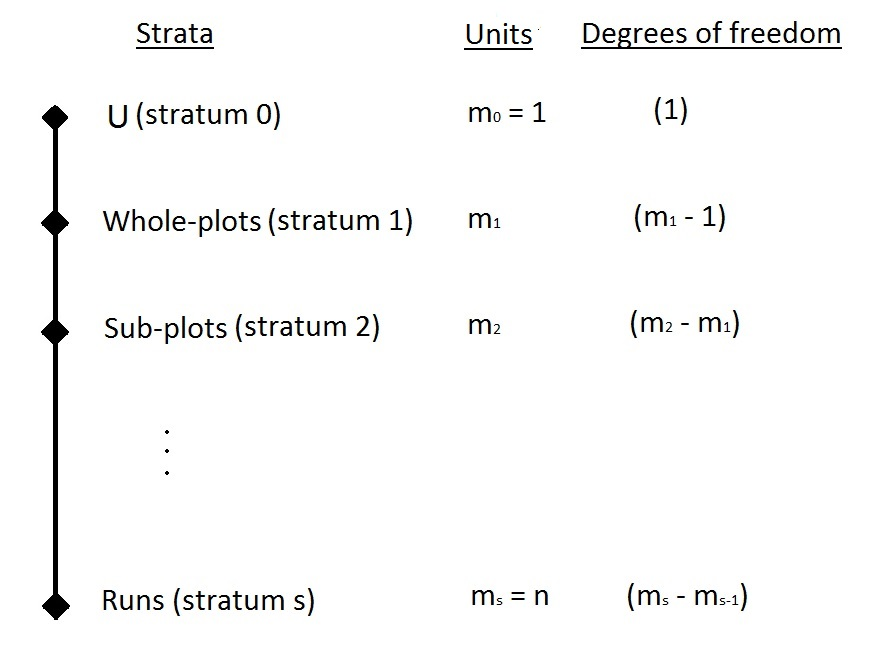
\includegraphics[scale=0.85]{Hasse.jpg}      %width=\textwidth
\caption{Hasse diagram for factors}
\label{Fig::Hasse}
\end{center}
\end{figure} 
 
Recall the expression for the linear polynomial hierarchical model from (\ref{eq::intro_ms}):
\begin{equation}
\label{eq::back_ms}
\bm{Y}=\bm{X}\bm{\beta}+\sum_{i=1}^{s}\bm{Z}_{i}\bm{\varepsilon}_{i},
\end{equation} 
where the first part $\bm{X\beta}$ contains the fixed effects, and $\sum_{i=1}^{s}\bm{Z}_{i}\bm{\varepsilon}_{i}$ stands for the random part, i.e.~it comprises information on variation occurring at each level of randomisation. All of the errors are assumed to be independent, having zero means and constant variances $\sigma^2_{i}$ and, as seen from the model formulation, additive.

In this case the fixed effects coefficients, $\bm{\beta}$ are usually estimated using the Generalised Least Square (GLS) formula:
\begin{equation}
\label{eq::back_gls}
\bm{\hat{\beta}}=(\bm{X}'\bm{VX})^{-1}\bm{X}'\bm{V}^{-1}Y,
\end{equation}
so that the variance of the estimators is
\begin{equation}
\label{eq::back_glsvar}
Var(\bm{\hat{\beta}})=(\bm{X}'\bm{VX})^{-1},
\end{equation}
where $\bm{V}$ is the variance-covariance matrix of the (normally distributed) responses, has a block-diagonal structure, and can be presented as:
\begin{equation}
\label{eq::back_glsV}
\bm{V}=\sum_{i=1}^{s}\sigma^2_{i}\bm{Z}_{i}\bm{Z}'_{i}=\sigma^{2}_{s}\left(\bm{I}_{n}+\sum_{i=1}^{s-1}\eta_{i}\bm{Z}_{i}\bm{Z}'_{i}\right).
\end{equation}
Here $\eta_{i}=\sigma^{2}_{i}/\sigma^{2}_{s}$ is defined as a variance ratio, denoting the magnitude of variability occurring at higher strata scaled with respect to the between-run variance.

At the analysis stage, as the variance components are unknown, their estimates are obtained and substituted in (\ref{eq::back_glsvar}) to obtain an estimated variance-covariance matrix of the parameters' estimators, $\bm{\hat{V}(\hat{\beta})}$; the estimation methods are discussed in more detail in Chapter \ref{ch::mse_ms}.

However, when an experiment is being planned, and none of the $\eta_{i}$ or $\sigma^2_{s}$ are known, there are two main approaches to deal with it. The first one is to search for designs assuming some point prior values of the $\eta$ parameter and, for these, evaluate the variance-based criteria, considering all strata simultaneously.

The case of split-plot experiments, with two strata, $\sigma^2_{s}=\sigma^2$ and $\eta=\sigma^2_{1}/\sigma^2$, has been extensively considered in the literature. \cite{Goos2001Doptimal} considered the three cases when D-optimal designs for split-plot experiments do not depend on the value of $\eta$; in other practical cases an estimate of the variance ratio is to be provided. \cite{Goos2003Doptimal} and \cite{Jones2007candidate} developed algorithms for finding $D$-optimal split-plot designs and for some examples demonstrated the robustness to the different values of $\eta$. An algorithm for constructing $D$-optimal split-split-plot designs can be found in the paper by \cite{Jones2009Doptimal}. 
%\cite{Goos2007tailor} -- split-plot for mixture experiments  

The Bayesian alternative to the `exhaustive search' approach across the unknown parameter space allows specifying a prior distribution on the unknown parameters, and then evaluating the criteria by integrating over that prior. \cite{Arnouts2012staggered} presented a coordinate-exchange algorithm for constructing D-optimal designs for a staggered experimental structure (i.e. values of hard-to-change factors' are changed at different time points), with log-normal prior distributions being put on the variance ratios. Later \cite{Arnouts2015staggered} studied the staggered structured designs in the context of response surface modelling, and considered a few examples of D- and I-optimal designs.
 
\cite{Mylona2014optimal} introduced a composite criterion, combining $D$-optimality for the fixed and variance components; in such an approach both the criterion formula and the form of the prior distributions define the way of evaluation the criterion function, which often leads to the necessity of choosing a computationally efficient numerical methodology. \cite{Gilmour2009analysis} proposed an appropriate Bayesian analysis strategy of data from multistratum experiments, that is robust to designs non-orthogonality and is shown to be more reliable than REML approach.  

However, in the general case a lot of computational effort might be required in order to be confident in the goodness of the design obtained by choosing from a set of assumed possible values of $\eta_i$, either using point priors or adapting general Bayesian strategy, especially when there are more than two strata and, therefore, the range of unknown parameters becomes multi-dimensional. The stratum-by-stratum approach (as first suggested by \cite{Trinca2001multistratum} and more recently improved by \cite{Trinca2015improved}) implies going from the highest stratum to the lowest, at each level choosing the set of treatments, and the units of higher level being treated as fixed block effects. Such methodology allows `protecting' against the case of large higher level variances, and eliminates the need for any prior information on unknown parameters. The authors later adapted the stratum-by-stratum  strategy for the inference criteria \citep{Trinca2016SPinference}, providing tools for constructing efficient designs for relatively small experiments in the presence of restricted randomisation.
\section{Acknowledgements}

%%% Bibliography
\cleardoublepage
\phantomsection
\addcontentsline{toc}{chapter}{Bibliography} 
%\bibliographystyle{apalike}
\bibliographystyle{rss}
\bibliography{thesis_bib}

\end{document}